
As a demonstration, we use Thompson sampling to optimize an unknown function $V(x)$ (the value function) using \gpmem.
%(\textbf{TODO} we should not assume $V$ is deterministic, it would be easy enough to make it random or have it give noisy samples.)
We assume $V$ is made available to Venture as a black-box.
The code for optimizing $V$ is given in Listing \ref{alg:bayesopt}.
For step \ref{itm:Thompson-conditioning} of Thompson sampling, the Bayesian update, we not only condition on the new data (the chosen action $a$ and the received reward $r$), but also perform inference on the hyperparameters $\sigma, \ell$ using a Metropolis--Hastings sampler.
These two inference steps take 1 line of code: 0 lines to condition on the new data (as this is done automatically by \gpmem), and 1 line to call Venture's built-in \texttt{MH} operator.
The results are shown in Figure \ref{fig:bayesopt-sequence}.
We can see from the figure that, roughly speaking, each successive probe point $a$ is chosen either because the current model $V_\emu$ thinks it will have a high reward, or because the value of $V_\emu(a)$ has high uncertainty.
In the latter case, probing at $a$ decreases this uncertainty and, due to the smoothing kernel, also decreases the uncertainty at points near $a$.
We thus see that our Thompson sampler simultaneously learns the value function and optimizes it.

\begin{minipage}{\linewidth}
\small
\belowcaptionskip=-10pt
\begin{lstlisting}[frame=single,caption={
  Code for Bayesian optimization using \gpmem.
  %The procedure \texttt{V\_compute} probes \texttt{V} directly, thus improving the GP model \texttt{V\_emu}.
  %(\texttt{V\_emu\_pointwise} is simply a shortcut for sampling the GP model at a single point; \texttt{V\_emu} is more general, allowing joint samples to be taken at any set of points.)
  In the loop, \texttt{V\_compute} is called to probe the value of \texttt{V} at a new argument.
  The new argument, \texttt{(mc\_argmax V\_emu\_pointwise mc\_sampler)}, is a Monte Carlo estimate of the maximum pointwise sample of \texttt{V\_emu} (itself a stochastic quantity), with the Monte Carlo samples being drawn in this case uniformly between $-20$ and $20$.
  After each new call to \texttt{V\_compute}, the Metropolis--Hastings algorithm is used to perform inference on the hyperparameters of the covariance function in the GP model in light of the new conditioning data.
  Once enough calls to \texttt{V\_compute} have been made (in our case we stopped at 15 calls), we can inspect the full list of probed $(a,r)$ pairs with \texttt{extract\_stats}.
  The answer to our maximization problem is simply the pair having the highest $r$; but our algorithm also learns more potentially useful information.},mathescape,numbers=none,label=alg:bayesopt]
assume sf = tag(quote(hyper), 0, uniform_continuous(0, 10))
assume l = tag(quote(hyper), 1, uniform_continuous(0, 10))
assume se = make_squaredexp(sf, l)
assume blackbox_f = get_bayesopt_blackbox()
assume (f_compute, f_emu) = gpmem(blackbox_f, se)

define get_uniform_candidate = proc(prev_xs) {
  uniform_continuous(-20, 20)
}

define mc_argmax = proc(func, prev_xs) {
  // Monte Carlo estimator for the argmax of func.
  run(do(
    candidate_xs <- mapv(proc(i) {get_uniform_candidate(prev_xs)},
                         linspace(0, 19, 20)),
    candidate_ys <- mapv(func, candidate_xs),
    lookup(candidate_xs, argmax_of_array(candidate_ys))))
}

define emulator_point_sample = proc(x) {
  run(sample(lookup(
    f_emu(array(x)),
    0)))
}

infer repeat(15, do(pass,
     // Phase 2: Call f_compute on the next probe point
     predict f_compute(
                 mc_argmax(emulator_point_sample, '_)),
     // Phase 1: Hyperparameter inference
     mh(quote(hyper), one, 50)))
\end{lstlisting}
\end{minipage}
      
\begin{figure}
\centering
    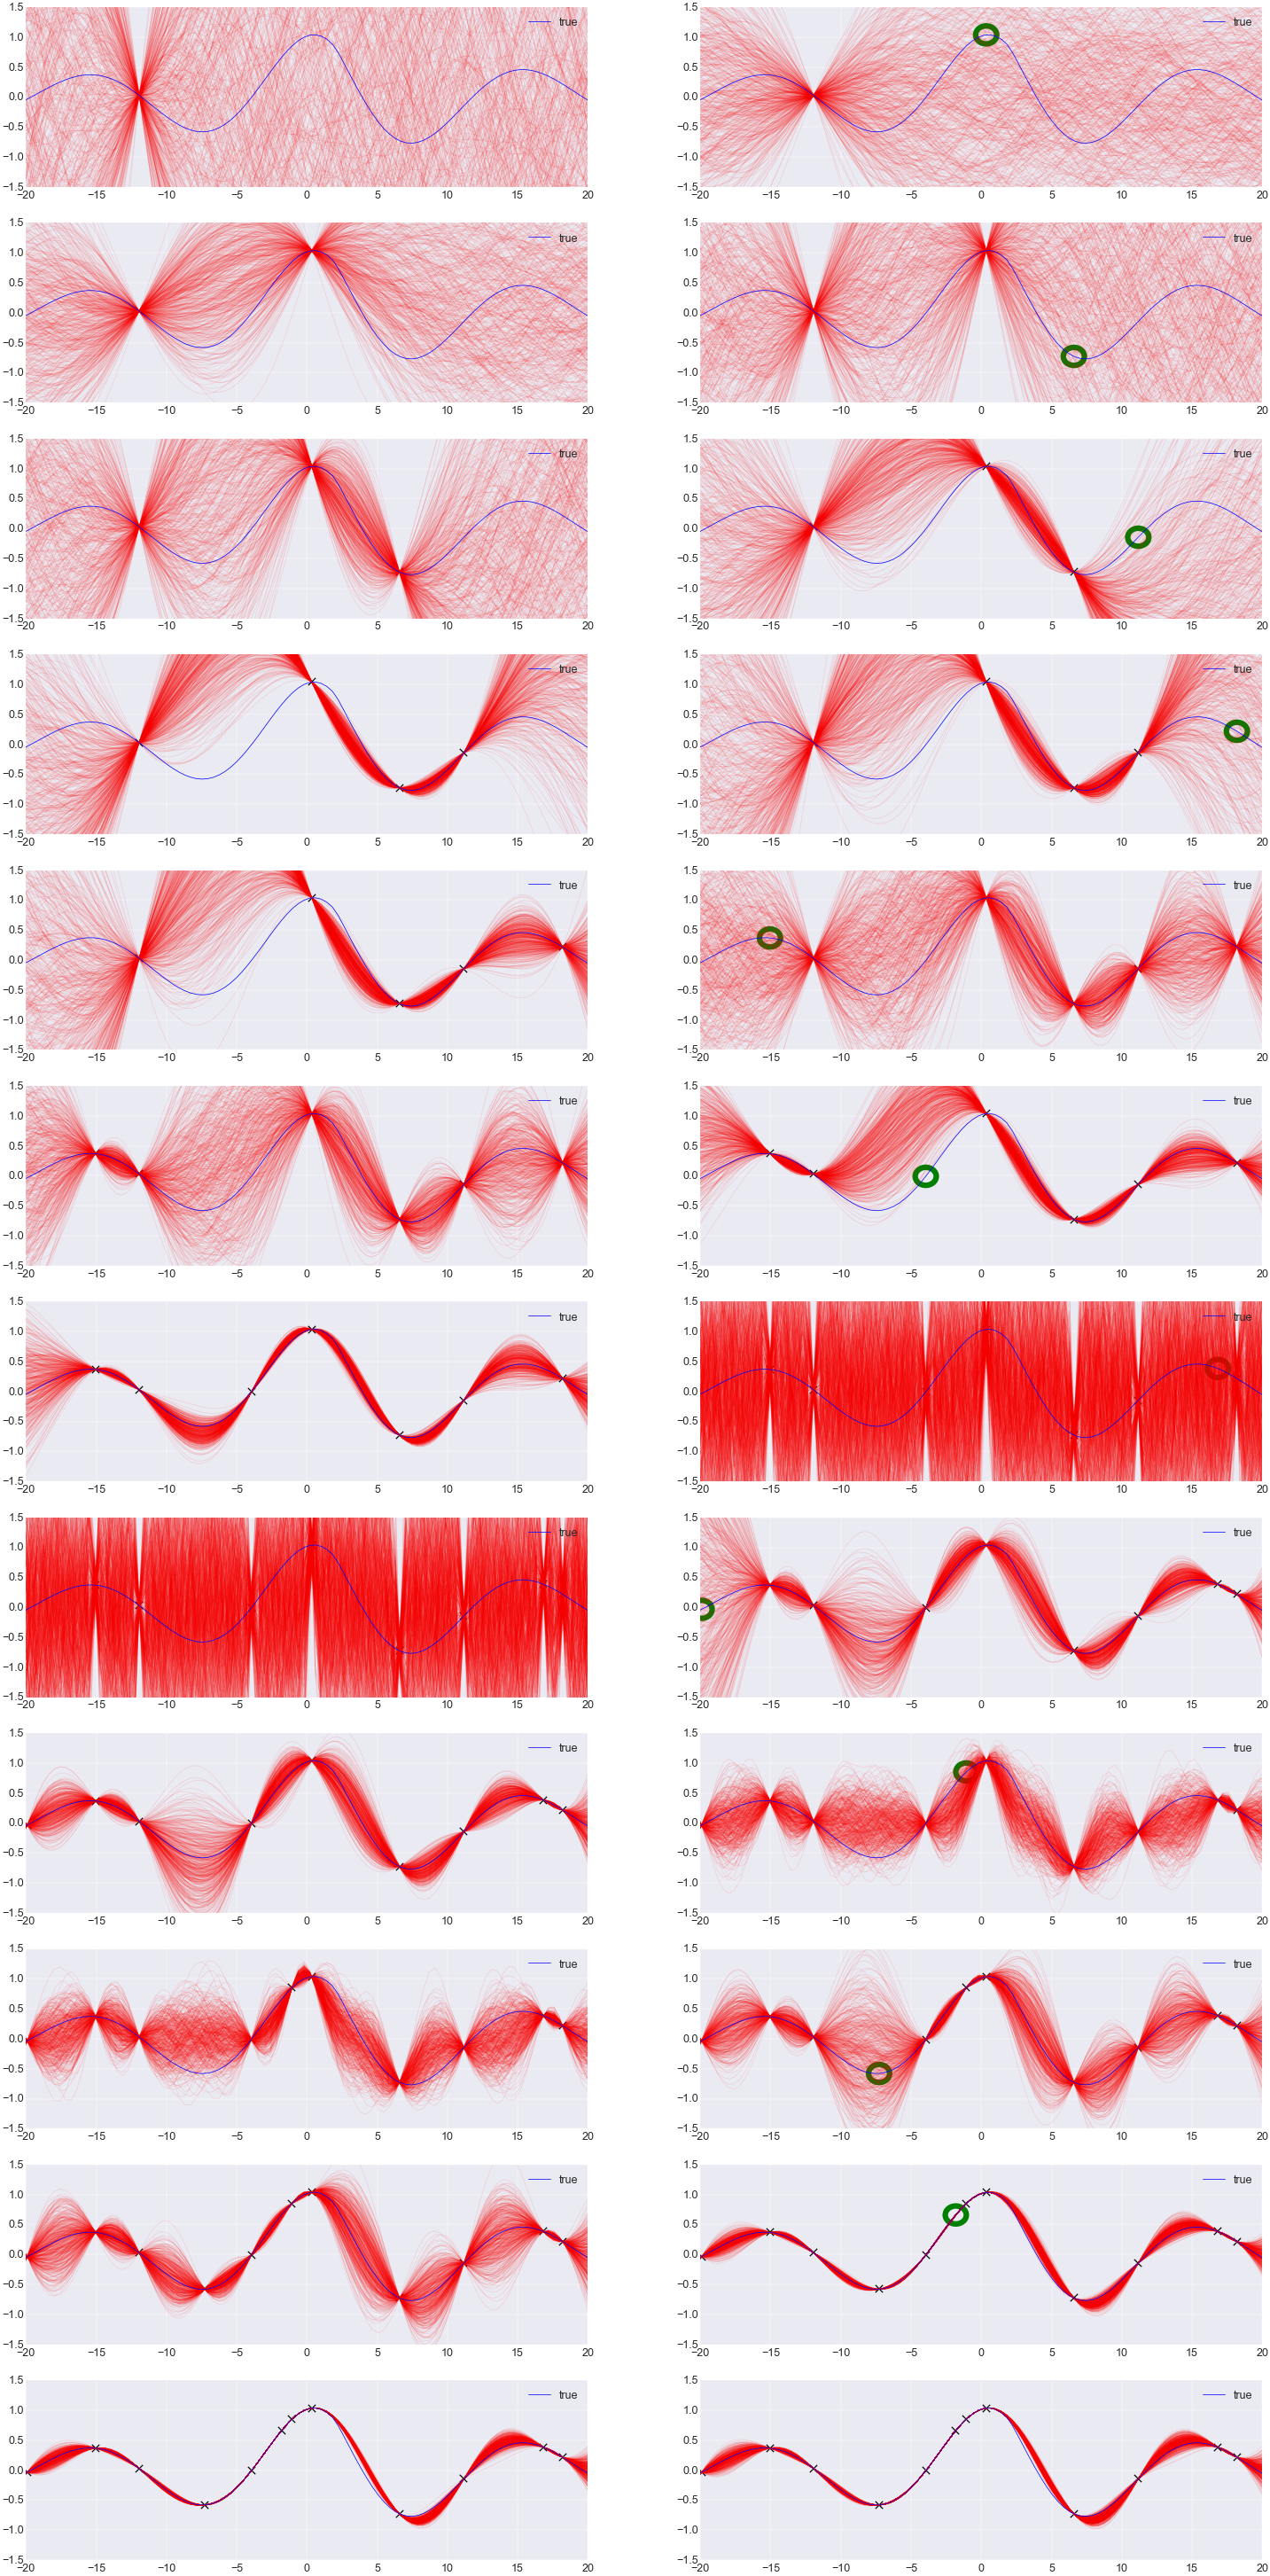
\includegraphics[height=0.8\textheight]{figs/BayesOpt_gpmem_sequence.png}
    \caption{
      Dynamics of Thompson sampling in Venture.
      The blue curve is the true function $V$, and the red region is a blending of 100 samples of the curve generated (jointly) by a GP-based emulator $V_\emu$.
      The left and right columns show the state of $V_\emu$ before and after hyperparameter inference is run on the new data, respectively.
      (We can see, for example, that after the seventh probe point, the Metropolis--Hastings sampler chose a ``crazy'' set of hyperparameters, which was corrected at the next inference step.)
      In the right column, the next chosen probe point is circled in green.
      Each successive probe point $a$ is the (stochastic) maximum of $V_\emu$, sampled pointwise and conditioned on the values of the previously probed points.
      Note that probes tend to happen at points either where the value of $V_\emu$ is high, or where $V_\emu$ has high uncertainty.
      }
    \label{fig:bayesopt-sequence}
\end{figure}



%We consider a true and  unknown reward function $r(x)$ that we estimate with a GP prior $\mathcal{GP}(0,K(\mathbf{x},\mathbf{x}))$. We denote past observations with $\mathcal{D} = \{(x;

\FloatBarrier
